\setmodule{10}

%BEGIN_FOLD % ====>>_____ Занятие 1 _____<<====
\begin{class}[number=1]
	\begin{listofex}
		\item Банка краски стоила \( 270 \) рублей. После подорожания она стала стоить на \( 20\% \) дороже. Сколько заплатит покупатель за \( 6 \) банок по новой цене?
		\item На клетчатой бумаге с клетками \( 1*1 \) см изображен треугольник. Найти его площадь квадратных сантиметрах.
		\begin{center}
			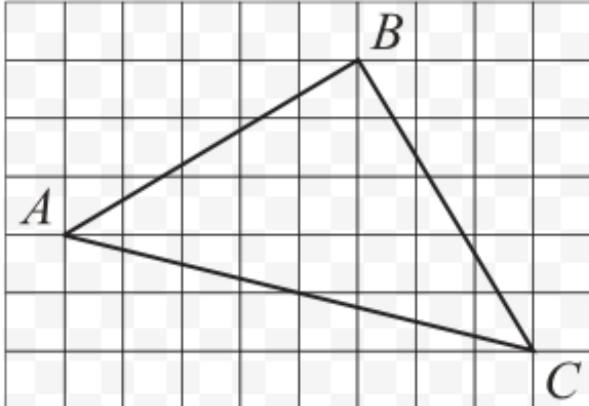
\includegraphics[align=t, width=0.5\linewidth]{../\picpath/MoisenkoL1}
		\end{center}
		\item Упростите выражение: \( \log_414-\log_47 \)
		\item Найдите значение выражения: \( 3\tg33\degree\cdot2\tg57\degree \)
		\item Решите уравнение: \( \sqrt{x^2-x-3}=3 \)
		\item Найдите корень уравнения. В случае, если их несколько, найдите их сумму: \( \log_2(x^2-3x+3)=0 \)
		\item Найдите значение выражения \( \tg\alpha-2\sin\alpha \), если \( \cos\alpha=0,8 \) и \\ \( \dfrac{3\pi}{2}\le\alpha\le2\pi \)
		\item Вычислите значение выражения: \( 2(\sqrt{x}-2)\cdot(\sqrt{x}+2) \), если \( x=6 \)
		\item Решите неравенство: \( 3^{x+3}<\dfrac{1}{27} \)
		\item Найдите область значения функции \( y=\sqrt{\dfrac{x+2}{2x-8}} \)
		\item В таксомоторной фирме \( 40 \) машин: \( 13 \) желтых, \( 12 \) черных. Остальные --- белые. Определить вероятность, что прибывшая по заказу машина не черная.
		\item Найдите точку минимума функции: \( y=x^3-18x+6 \)
		\item Найдите объём \( V \) конуса, образующая которого равна \( 3 \) и наклонена к плоскости основания под углом \( 30\degree \). В ответ укажите \( \dfrac{V}{\pi} \).
		\item Дана правильная четырёхугольная пирамида. Сторона основания равна \( 6 \). Высота равна \( 4 \). Найдите синус угла наклона бокового ребра к основанию пирамиды.
		\item Решите уравнение \( \cos\left( \dfrac{\pi}{4}-10x \right)=0 \)
		\item В правильной треугольной призме со стороной основания \( 6 \) и высотой \( 4 \) проведено сечение через сторону нижнего основания и противоположную вершину верхнего основания.
		Определить площадь сечения.
		\item Решите систему неравенств:
		\( \begin{cases} \dfrac{9^x-1}{3-3^x}<0 \\ \log_2(x+2)\le1 \end{cases} \)
	\end{listofex}
\end{class}
%END_FOLD

%BEGIN_FOLD % ====>>_____ Занятие 2 _____<<====
\begin{class}[number=2]
	\begin{listofex}
		\item .
	\end{listofex}
\end{class}
%END_FOLD

%BEGIN_FOLD % ====>>_ Домашняя работа 1 _<<====
\begin{homework}[number=1]
	\begin{listofex}
		\item Решите системы неравенств:
		\begin{tasks}(2)
			\task \( \begin{cases} \dfrac{7^x-49}{7-7^x}<0 \\ \log_2(x+6)\ge0 \end{cases} \)
			\task \( \begin{cases} \dfrac{6^x-216}{36-6^x}\le0 \\ \log_{\dfrac{1}{9}}(x-6)<0 \end{cases} \)
		\end{tasks}
		\item Решите уравнения: 
		\begin{tasks}(2)
			\task \( \sin\dfrac{\pi x}{3}=0,5 \)
			\task \( \cos\dfrac{\pi(x+1)}{4}=\dfrac{\sqrt{2}}{2} \)
		\end{tasks}
		\item Найдите первообразную функции:
		\begin{tasks}(3)
			\task \( y=4x^5 \)
			\task \( y=4 \)
			\task \( y=x^2+2 \)
		\end{tasks}
	\end{listofex}
\end{homework}
%END_FOLD

%BEGIN_FOLD % ====>>_____ Занятие 3 _____<<====
\begin{class}[number=3]
	\begin{listofex}
		\item ю
	\end{listofex}
\end{class}
%END_FOLD

%BEGIN_FOLD % ====>>_____ Занятие 4 _____<<====
\begin{class}[number=4]
	\begin{listofex}
		\item Занятие 4
	\end{listofex}
\end{class}
%END_FOLD

%BEGIN_FOLD % ====>>_ Домашняя работа 2 _<<====
\begin{homework}[number=2]
	\begin{listofex}
		\item Домашняя работа 2
	\end{listofex}
\end{homework}
%END_FOLD

%BEGIN_FOLD % ====>>_____ Занятие 5 _____<<====
\begin{class}[number=5]
	\begin{listofex}
		\item Занятие 5
	\end{listofex}
\end{class}
%END_FOLD

%BEGIN_FOLD % ====>>_____ Занятие 6 _____<<====
\begin{class}[number=6]
	\begin{listofex}
		\item Найдите значение выражения:
		\begin{tasks}(4)
			\task \( \sin210\degree \)
			\task \( \cos240\degree \)
			\task \( \cos300\degree \)
			\task \( \sin330\degree \)
			\task! \( 2\cdot\tg33\degree\cdot\ctg33\degree \)
		\end{tasks}
		\item Найдите:
		\begin{tasks}(1)
			\task \( \sin\alpha \), если \( \cos\alpha=-0,6 \) и \( 180\degree<\alpha<270\degree \)
			\task \( \sin\alpha \), если \( \cos\alpha=-0,8 \) и \( 90\degree<\alpha<180\degree \)
			\task \( \sin\alpha \), если \( \cos\alpha=\dfrac{\sqrt{3}}{2}\) и \( 270\degree<\alpha<360\degree \)
			\task \( 2\cdot\cos^2\alpha \), если \( \sin\alpha=-0,2 \)
		\end{tasks}
		\item Найдите значение выражения:
		\begin{tasks}(2)
			\task \( \sqrt{0,02}\cdot\sqrt{0,18} \)
			\task \( 10\cdot\sqrt{0,1}\cdot\sqrt{0,004} \)	
			\task \( \left( \sqrt{\dfrac{3}{2}}-1 \right)\left( \sqrt{\dfrac{3}{2}}+1 \right) \)
			\task \( (\sqrt{17}-2\sqrt{3})(\sqrt{17}+2\sqrt{3}) \)
			\task \( (2\sqrt{5}-4)(4+2\sqrt{5}) \)
			\task \( (3\sqrt{2}-2\sqrt{3})(2\sqrt{3}+3\sqrt{2}) \)
			\task \( \left( 2\sqrt{\dfrac{1}{2}}-2 \right)\left( 2\sqrt{\dfrac{1}{2}}+2 \right) \)
		\end{tasks}
	\end{listofex}
\end{class}
%END_FOLD

%BEGIN_FOLD % ====>>_ Домашняя работа 3 _<<====
\begin{homework}[number=3]
	\begin{listofex}
		\item Домашняя работа 3
	\end{listofex}
\end{homework}
%END_FOLD

%BEGIN_FOLD % ====>>_____ Занятие 7 _____<<====
\begin{class}[number=10]
	\begin{listofex}
		\item Найдите наименьшее значение функции \( \dfrac{x^3}{3}-9x-7 \) на отрезке \( [-3;3] \).
		\item Найдите объём конуса, образующая которого равна \( 44 \) и наклонена к плоскости основания под углом \( 30\degree \). В ответ запишите объём, делённый на \( \pi \).
		\item Боковые ребра правильной четырехугольной пирамиды равны \( 5 \), сторона основания равна \( 8 \). Найдите площадь поверхности пирамиды.
		\item Решите уравнение: \( \cos\dfrac{\pi(x-7)}{3}=\dfrac{1}{2} \).
		\item В правильной четырехугольной призме через диагональ основания проведено сечение параллельно диагонали призмы. Найдите площадь сечения, если сторона основания призмы равна \( 2 \) см, а ее высота равна \( 4 \) см.
		\item Решите систему неравенств:
		\( \begin{cases} \dfrac{5^x-1}{5-5^x}<0 \\ \log_3(x+1)\le0 \end{cases} \)
		\item Найдите промежутки убывания функции: \( f(x)=12x+3x^2-2x^3 \).
	\end{listofex}
\end{class}
%END_FOLD

%BEGIN_FOLD % ====>>_ Проверочная работа _<<====
\begin{exam}
	\begin{listofex}
		\item Проверочная
	\end{listofex}
\end{exam}
%END_FOLD